\documentclass[11pt]{ctexart}

\usepackage{multicol}
%\usepackage{mwe}
\usepackage{subfigure}
\usepackage{mathtools}
\usepackage{graphicx}
\usepackage{amsmath}
\usepackage{mathrsfs}
\usepackage[top=0.5in,bottom=1in,left=1in,right=1in]{geometry}
\usepackage{pdflscape}
\usepackage{times}
\usepackage{bm}
%\usepackage{setspace}
\usepackage{color}
\usepackage{caption}
\usepackage{amsmath}
\usepackage{amssymb}
\usepackage{CJK}
\usepackage{longtable}
%\usepackage[final]{pdfpages}
\usepackage{listings}
\usepackage{textcomp}
\usepackage{xcolor}
\usepackage{algorithm2e}
\usepackage{float}
\usepackage{algorithmicx}
\usepackage{algpseudocode}
\usepackage{hyperref}

\hypersetup{hidelinks,
	colorlinks=true,
	allcolors=black,
	pdfstartview=Fit,
	breaklinks=true}

\pagestyle{plain}




\begin{document}

\title{第十八周实习报告20220715}
\author{宋欣源}
\date{\today}

\maketitle % need full-width title

\CTEXsetup[format={\Large\bfseries}]{section}

\section{第一,综述}

下面对于这些天实习的工作做一个报告。现在就这一周的工作做一个总结
我这周主要在raw3和 \par raw4数据集上进行。主要是研究resnet,从resnet10到resnet30到resent50的网络

\section{第二,resnet50模型和实验}
\subsection{综述}
resnet的结构就是residual,有多种结构,如下图:
\begin{figure}[H]

\begin{center}
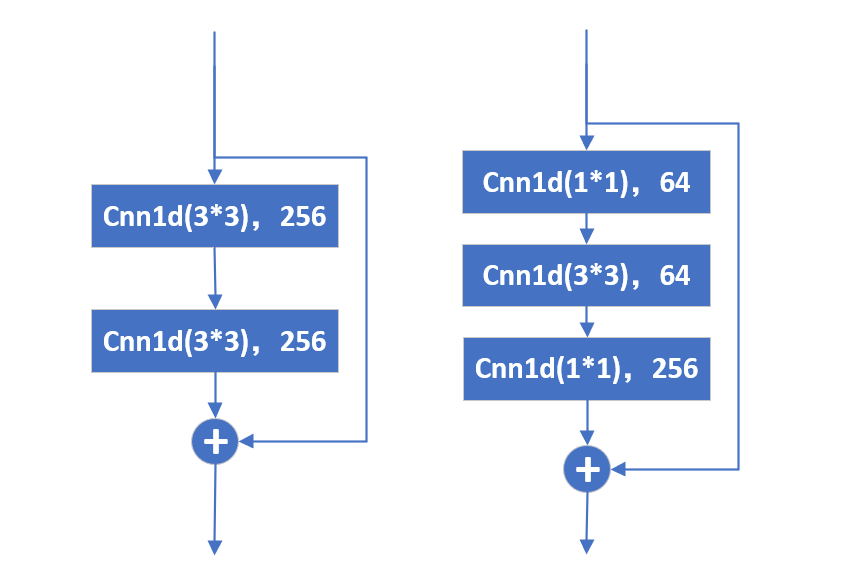
\includegraphics[width=0.9\textwidth]{residual1.PNG}
\end{center}
\caption{residual structure}
\label{FIG.1}
\end{figure}

按照这两种结构进行堆叠,成如下的结构,把这种结构在上面的30层cnn1d上进行应用,如图:
\begin{figure}[H]

\begin{center}
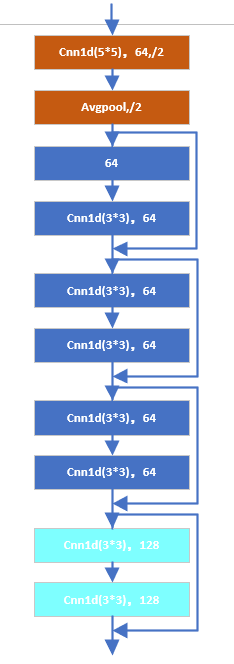
\includegraphics[width=0.4\textwidth]{residual2.PNG}
\end{center}
\caption{residual cnn1d30 structure}
\label{FIG.2}
\end{figure}

加入了residual,具体的细节结构还需要进一步尝试,究竟shortcut是插入在avg之中,relu之中还是batchnorm以后。以及resnet50的residual结构都在上面的30层cnn1d上进行应用。得到如下的的模型。

~\\
模型1:Resnet3(256)

这个模型是3层resnet,hidden\_size是256的模型,采用了两种

模型表现{\kaishu \small IC: 0.065, pnl:2.677}

~\\
模型2:Resnet5(64-256)

这个模型是5层resnet,hidden\_size是256的模型,采用了两种residual的形式.目前模型收敛速度很快,过拟合可能性较高。在这方面进行探索。

模型表现{\kaishu \small IC: 0.066, pnl:2.689}

~\\
模型3:Resnet10(64-256)

这个模型是10层resnet,hidden\_size是64到256的模型,效果有一定的退化,但是收敛速度下降了,继续加深深度。

模型表现{\kaishu \small IC: 0.068, pnl:2.604}


经过上面的研究,取得了不错的效果,但是效果还不够。因此又做了大量尝试,结果都差不多。直接想到应该继续加深模型,有了以下这些模型结果

~\\
模型4:Resnet13(64-128-256)

这个模型是13层resnet,hidden\_size是64到128到256的模型。模型进行了判断,当遇到 \par hidden\_size变化的时候,不加resnet,其他情况加上。另外都加上batchnorm和dropout

模型表现{\kaishu \small IC: 0.068, pnl:2.660}

~\\
模型5:Resnet20(64-128-256-512)

这个模型是20层resnet,hidden\_size是64到128到256到512的模型。模型进行了判断,当遇到 \par hidden\_size变化的时候,不加resnet,其他情况加上。另外都加上batchnorm和dropout

模型表现{\kaishu \small IC: 0.069, pnl:2.703}

~\\
模型6:Resnet30(64-128-256-256-512)

这个模型是30层resnet,hidden\_size是64到128到256到512的模型。经过大量实验,256维度最适合24维度输入的raw3和raw4。因此在256的维度上再做一次resnet。维度升高又有过拟合的问题

模型表现{\kaishu \small IC: 0.071, pnl:2.735}

~\\
模型7:Resnet30(64-128-256-256-512-avgpool)

经过大量实验,模型一直在附近徘徊,而且稳定性不够好。所以尝试利用stride和avgpool进行尺度缩进,尺度逐渐缩短,让卷积极可能的暴露在外面。首先尝试一次avgpool,模型有进步

模型表现{\kaishu \small IC: 0.066, pnl:2.746}

~\\
模型8:Resnet30(64-128-256-256-avgpool-512-avgpool)

做两次avgpool,注意avgpool一定要放在最后,不能平均放置。

模型表现{\kaishu \small IC: 0.062, pnl:2.665}

~\\
模型9:Resnet30(64-avgpool-128-avgpool-256-256-avgpool-512-avgpool)

四次avgpool以后,模型过拟合程度有了改善。一般要三四个epoche维持在峰值附近。但是效果一直一般。仔细想想出现的原因,可能是目前的两种residual解释力不够。另外residual直接shortcut,很容易造成不训练直接走捷径的信息流。要想办法提高卷积所占的比例。初步的想法是给shortcut也加上卷积。

模型表现{\kaishu \small IC: 0.063, pnl:2.651}

因此,在residual的shortcut上也加上卷积,batchnorm和avgpool,在两条路径上进行优化。最简单的方式就是如下这种:

\begin{figure}[H]

\begin{center}
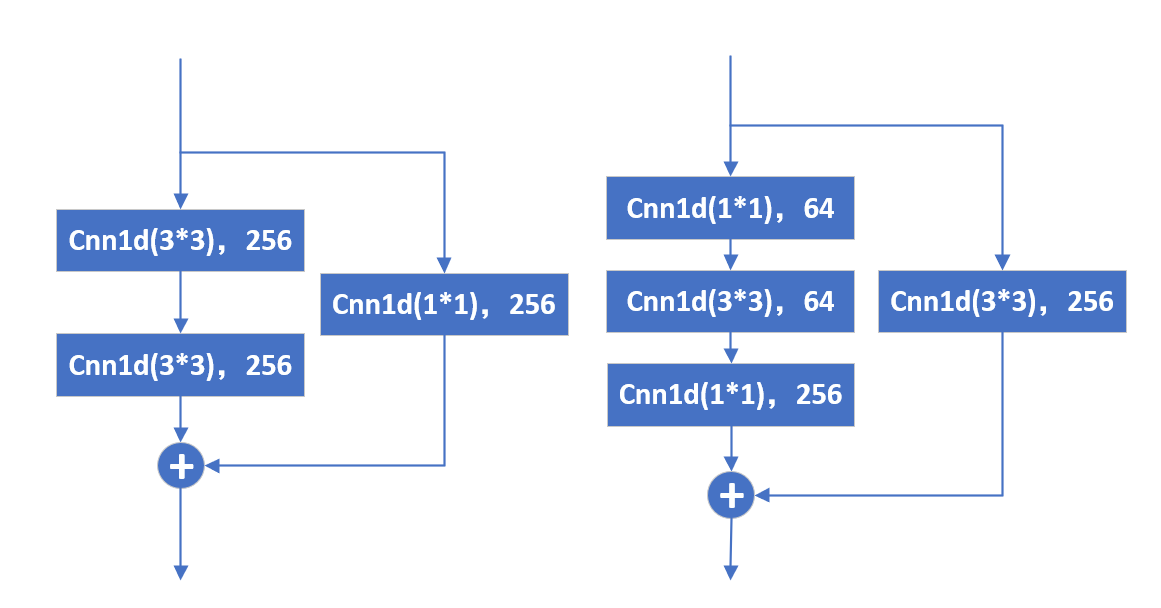
\includegraphics[width=1.0\textwidth]{residual3.PNG}
\end{center}
\caption{residual structure\_v2}
\label{FIG.3}
\end{figure}

这种改造的好处是在侧路也加上卷积和avgpool,让几条信息流都有信息处理的结果,对resnet的实验也从13层开始,层数较低的在原来的实验中已经很多展示。

~\\
模型10:Resnet13\_v2(64-128-256)

13层简单模型上有所下降,经过观察,原因是侧边路更容易过拟合,得到纬度较低的模型。因此在shortcut路径上添加avgpool和dropout来控制shortcut的结果。

模型表现{\kaishu \small IC: 0.061, pnl:2.543}

~\\
模型11:Resnet13\_v2(64-128-256)

经过大量实验,在avgpool和batchnorm上做文章能达到这个程度。但是稳定性有所下降,因此减少relu的使用,让模型缓慢下降。取消residual之间的relu,只保留每一个residual  block的relu进行尝试。最后下降速度有所放缓,同时表现没有多少降低。

模型表现{\kaishu \small IC: 0.067, pnl:2.777}

~\\
模型12:Resnet20\_v2(64-128-256-512)

这个模型是20层resnet,hidden\_size是64到128到256到512的模型。模型还是有所下降。20层的实验难度比13层大很多。不能保证实验出优秀解法。经过大量实验,获得的模型普遍比现在情况低。因此先继续加深。

模型表现{\kaishu \small IC: 0.059, pnl:2.582}

~\\
模型13:Resnet30\_v2(64-128-256-256-512)

这个模型是30层resnet,hidden\_size是64到128到256到512的模型。把模型的维度提高到30层和 \par 20层效果很近,猜测是多出来的十层没有参与训练。因此在这十层上给模型找麻烦。首先是加入avgpool减少relu

模型表现{\kaishu \small IC: 0.059, pnl:2.583}

~\\
模型14:Resnet30\_v2(64-128-256-256-avgpool-512-avgpool)

找麻烦以后,模型效果有所提高,经过参数查看,发现这十层通过shortcut进行训练。那么采用同样的办法,修改shortcut模型,加入avgpool和dropout,现在的模型顺序为cnn1d-batchnorm-avgpool-dropout。去掉cnn1d和batchnorm之间的relu

模型表现{\kaishu \small IC: 0.061, pnl:2.639}

~\\
模型15:Resnet30\_v2(64-128-256-avgpool-256-avgpool-512-avgpool)

在20层和30层的链接点下功夫,实验了各种组合。达到相对于20层有所提高,模型表现回到2.70,说明30曾模型能表达20曾模型。同时降低拟合速度。

模型表现{\kaishu \small IC: 0.068, pnl:2.720}

~\\
模型16:Resnet30\_v2(64-128-avgpool-256-avgpool-256-avgpool-512-avgpool)

加入全部四个avgpool以后,实验的维度很多,经过大量实验,没找到实质性提高的办法。

模型表现{\kaishu \small IC: 0.066, pnl:2.714}

经过大量实验。可以实验的维度太多,都没有实质性的提高,因此,对residual block进行修改。最直接的想法是,将一条main和一条shortcut拆分成多个通路,拆分成32个通路,因此,每个通路的实际训练维度是4,groups设置为hidden\_dim//4,利用新的blocks进行训练。新的blocks形式如下:

\begin{figure}[H]

\begin{center}
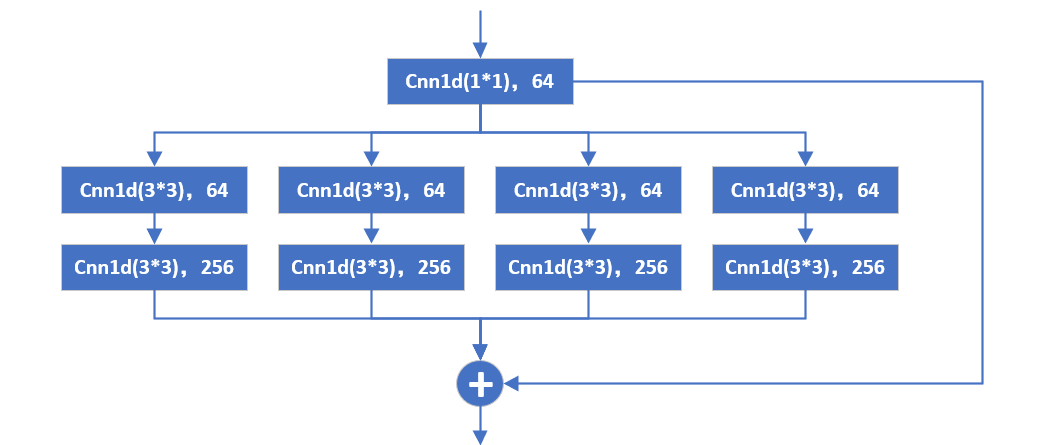
\includegraphics[width=1.0\textwidth]{residual4-1.PNG}
\end{center}
\caption{residual structure\_v3-1}
\label{FIG.4}
\end{figure}

\begin{figure}[H]

\begin{center}
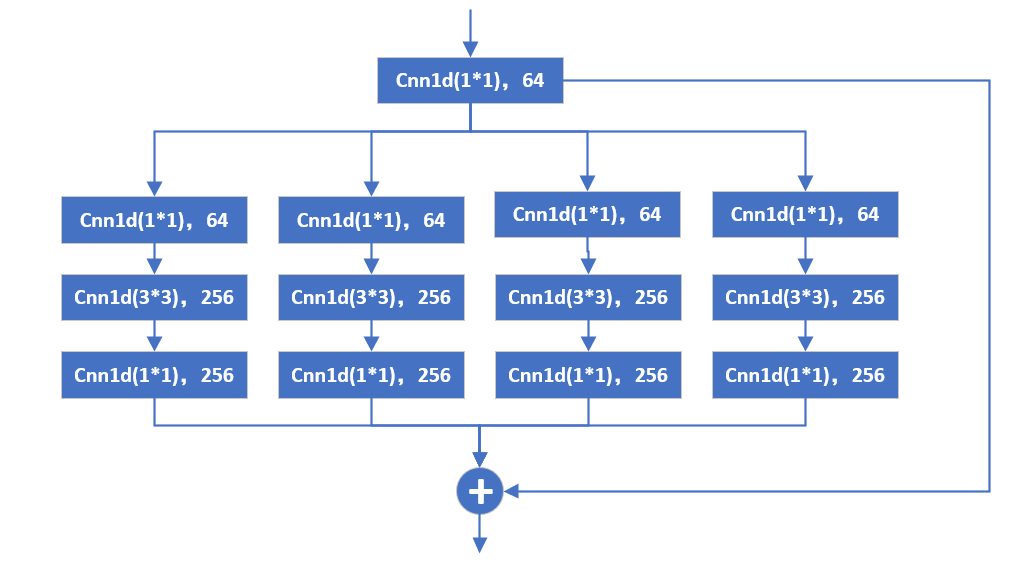
\includegraphics[width=1.0\textwidth]{residual4-2.PNG}
\end{center}
\caption{residual structure\_v3-2}
\label{FIG.5}
\end{figure}

在这个基础上,仍然是在13层以上模型上进行试验。

~\\
模型17:Resnet13\_v3-1(64-128-256)

13层简单模型上有所下降,在这个多通路模型中,不存在某条路容易信息容易行走的情况。容易进行实验。在此基础上进行加深。

模型表现{\kaishu \small IC: 0.062, pnl:2.576}

~\\
模型18:Resnet13\_v3-2(64-128-256)

经过大量实验,groups=1的模型下降速度较慢,同时最终结果较好

模型表现{\kaishu \small IC: 0.067, pnl:2.777}

~\\
模型19:Resnet20\_v3-2(64-128-256-512)

这个模型是20层resnet,hidden\_size是64到128到256到512的模型。模型还是有所下降。20层的实验难度比13层大很多。不能保证实验出优秀解法。经过大量实验,获得的模型普遍过拟合现象比较严重。

模型表现{\kaishu \small IC: 0.066, pnl:2.771}

~\\
模型20:Resnet30\_v3-2(64-128-256-256-512)

这个模型是30层resnet,hidden\_size是64到128到256到512的模型。利用前面的经验同样的方法进行修改,由于blocks具有更多参数,大量实验的结果普遍在2.7以上,加入各类avgpool和relu和 \par batchnorm来降低过拟合速度。


模型表现{\kaishu \small IC: 0.069, pnl:2.756}

~\\
模型21:Resnet30\_v3-2(64-128-256-avgpool-256-avgpool-512-avgpool)

相比而言,v3-2模型比v3-1模型稍好一些,主要体现在过拟合速度上,同时观察weight的分布,具有更少的极端情况,在实际操作中体现出换手率较低的特点。

模型表现{\kaishu \small IC: 0.069, pnl:2.748}

~\\
模型22:Resnet30\_v3-1(64-128-256-avgpool-256-avgpool-512-avgpool)

基于v3-1的backbone,实验了各种组合。将dropout取消,加入更多的batchnorm来减少极端值的情况,效果有所改善。

模型表现{\kaishu \small IC: 0.068, pnl:2.694}

~\\
模型23:Resnet30\_v3-2(64-128-avgpool-256-avgpool-256-avgpool-512-avgpool)

加入全部四个avgpool以后,实验的维度很多,需要经过大量实验,目前是稳定在2.7左右,同时能在2.6坚持4-5个epoche。

模型表现{\kaishu \small IC: 0.069, pnl:2.714}

经过大量实验,可以实验的维度太多,从直观感受上,不缩并的模型,很难采用到每一层每一个参数。目前的缩并是通过avgpool来池化进行缩并。所以很容易想到利用cnn1d的stride进行缩并。原来的模型中已经有很多很好的尝试。积累了一些经验,现在不妨将residual的stride设置为2,和avgpool一起缩并,保证residual都完整训练,不会存在信息直达的通路。模型基于residual structure\_v2进行改进,结构图如下:
\begin{figure}[H]

\begin{center}
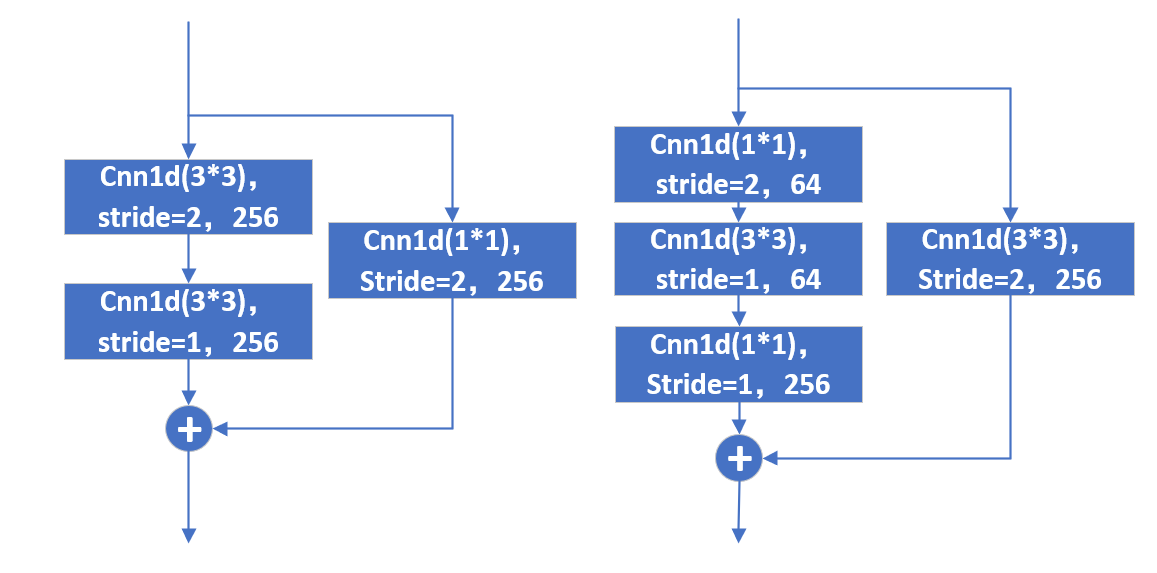
\includegraphics[width=1.0\textwidth]{residual5.PNG}
\end{center}
\caption{residual structure\_v4}
\label{FIG.6}
\end{figure}

改进后的模型,由于cnn1d已经开始参与收缩,所以深度不能很深,在13层以内。结果如下:

~\\
模型23:Resnet3(256)

这个模型是3层resnet,hidden\_size是256的模型,采用了两种结构的residual,最简单的模型也具有较好结果

模型表现{\kaishu \small IC: 0.068, pnl:2.691}

~\\
模型24:Resnet5(64-256)

这个模型是5层resnet,hidden\_size是256的模型,采用了两种residual的形式.IC提高很多,\par stride对整个模型影响较大,继续加深模型深度

模型表现{\kaishu \small IC: 0.071, pnl:2.763}

~\\
模型25:Resnet10(64-256)

这个模型是10层resnet,hidden\_size是64到256的模型,效果进一步提高,同时保持了很大程度的抗过拟合性质,在10层中,avgpool不再进行尺缩,采用cnn1d进行6次缩短,刚好能生成一个序列的观点。模型参数较大,但是整个模型都收到了充分地训练。在此基础上继续加深

模型表现{\kaishu \small IC: 0.073, pnl:2.805}

经过上面的研究,取得了不错的效果,但是效果还不够。因此又做了大量尝试,结果都差不多。直接想到应该继续加深模型,有了以下这些模型结果

~\\
模型26:Resnet13(64-128-256)

这个模型是13层resnet,hidden\_size是64到128到256的模型。模型进行了7次缩短,从weight的分布和训练程度看,每一个epoche模型都有显著变化。同时并没有太多极端数值的产生,IC也有所提高。模型表现也有所提高。结果如图所示。

模型表现{\kaishu \small IC: 0.079, pnl:2.875}

\begin{figure}[H]

\begin{center}
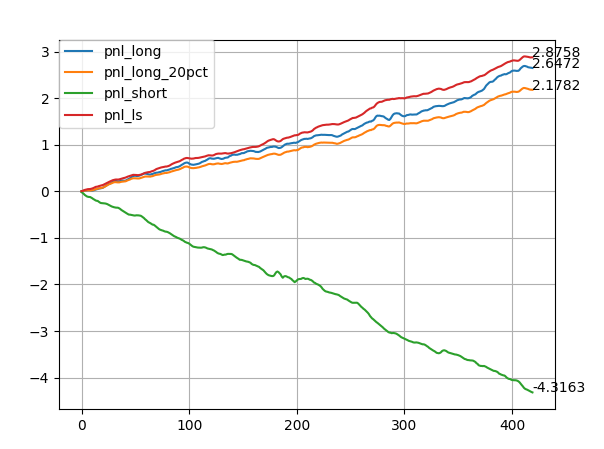
\includegraphics[width=0.8\textwidth]{result.PNG}
\end{center}
\caption{resnet13\_model26\_result}
\label{FIG.7}
\end{figure}

~\\
模型27:Resnet13(64-128-256)

这个模型是13层resnet,hidden\_size是64到128到256的模型。对模型进行了修改,加入了dropout, \par bias等参数,实验的方法有很多,寻找过拟合情况最好的模型

模型表现{\kaishu \small IC: 0.077, pnl:2.860}

~\\
模型28:Resnet13(64-128-256)

这个模型是13层resnet,hidden\_size是64到128到256的模型。每一层都采用尺缩,效果有所退化。原因是参数减少,导致最终很多层实际上只有一个参数点。所以这种residual\_blocks出现在合适的位置上最为关键。

模型表现{\kaishu \small IC: 0.072, pnl:2.760}

经过这些实验,采用了利用residual\_blocks代替cnn的做法。这种做法的模型更加稳健,效果和cnn1d的同深度的模型差不多,但是抗过拟合效果变好。在参数weight中异常的数值更少,每一层的下降更加缓慢平滑,具有良好模型的特点。因此后面用residual\_blocks进行组合研究。由于stride能使模型尺缩,整个模型训练得更充分,不存在某一部分数值训练较多的情况。因此后面的思路就是将含有尺缩的residual\_blocks和普通多通路的residual\_blocks进行组合。利用之前的经验进行替换。形成下一步的residual\_NEXT模型。这一部分研究主要是找到了能让模型变好的两条路。这两条路放在一起,进行下一步研究。另外resnet的特点是路径较多,信息流复杂,保证每一部分均匀的训练,需要格外注意。


\subsection{改进思路}
\begin{itemize}
  \item [0)]
    首先,residual深度还可以加深,加深后20层和30层的结构还可以细节上进行调整,还有很多实验的维度。目前常用的residual\_net都是50层以上,还有很多200层,低层的residual模型不能很好体现residual的特性,还需要进一步加深。
  \item [1)]
    residual的结构还可以进一步创新,做到稳定性和表现同步提高,拟合和去过拟合一起提高。下一步要研究residualNEXT模型就是在去过拟合上进行改进rsidual\_net。在stride,groups上已经做了很多,还可以进一步实验。另外,在bias=True或者False上不同的时候有不同的情况,这个细节还需要大量实验
  \item [2)]
    目前实验了8种residual\_blocks的格式,实验深度在30-35层,还有集中额外的residual\_blocks的结构,实验深度尝试达到50层可以进一步进行。不过我下一步首先训练residual\_NEXT网络。
\end{itemize}


\end{document} 